% ==========================================
% BAB V RENCANA SELANJUTNYA
% ==========================================
\chapter{RENCANA SELANJUTNYA}
\label{chap:rencana-selanjutnya}

\section{Rencana Implementasi}
Rencana implementasi dalam tugas akhir ini disusun berdasarkan model \textit{Software Development Life Cycle} (SDLC) Waterfall yang dipadukan dengan prinsip \textit{User-Centered Design} (UCD) pada tahap perancangan. Implementasi dilakukan secara terstruktur dan berurutan, di mana setiap tahap menghasilkan artefak yang menjadi dasar bagi tahap berikutnya. Fokus utama tugas akhir ini adalah pengembangan modul rekomendasi \textit{People-to-People} berbasis \textit{Affinity-Based Matching}, yang akan diintegrasikan dengan modul lain dalam platform kolaborasi mahasiswa. Tahap implementasi yang direncanakan adalah sebagai berikut.

\begin{enumerate}
\item {Tahap Detailisasi Desain dan Pemodelan Sistem} 
Tahap pertama adalah detailisasi desain dan pemodelan sistem, yang berfokus pada perumusan kebutuhan pengguna dan pendefinisian struktur sistem secara komprehensif. Pada tahap ini dilakukan penyusunan use case untuk seluruh interaksi pada modul \textit{People-to-People}, pemetaan alur proses pencocokan dari input profil hingga penyajian rekomendasi, serta pembuatan class diagram yang menggambarkan struktur data atribut pengguna seperti minat, kemampuan teknis, pengalaman, dan preferensi gaya kerja. Selain itu, dibuat pula wireframe awal sebagai bagian dari proses UCD untuk memvalidasi kebutuhan pengguna dan memastikan rancangan antarmuka sesuai dengan konteks penggunaan. Hasil dari tahap ini berupa blueprint desain modul rekomendasi yang akan menjadi acuan utama pada tahap implementasi selanjutnya.

\item {Tahap Pengembangan Antarmuka dan Modul Interaksi Pengguna}
Tahap kedua adalah pengembangan antarmuka dan modul interaksi pengguna, yang bertujuan membangun tampilan dan pengalaman pengguna pada fitur \textit{People-to-People}. Proses ini mencakup pembuatan mockup dan prototipe antarmuka yang merepresentasikan elemen-elemen utama seperti halaman \textit{feed} rekomendasi, tampilan profil mahasiswa lain, serta fitur interaksi seperti \textit{save profile} dan \textit{express interest}. Implementasi \textit{frontend} dilakukan dengan menjaga konsistensi gaya desain terhadap modul lain dalam platform, yaitu modul \textit{People-to-Project} dan \textit{Team Formation}, sehingga memberikan pengalaman yang terpadu bagi pengguna. Pada akhir tahap ini diperoleh antarmuka fungsional yang siap diintegrasikan dengan logika perhitungan \textit{affinity}.

\item {Tahap Pengembangan Engine Rekomendasi \textit{People-to-People}}
Tahap ketiga merupakan inti dari tugas akhir ini, yaitu pengembangan engine rekomendasi \textit{People-to-People} berbasis \textit{Affinity-Based Matching}. Pada tahap ini dilakukan penentuan atribut profil yang digunakan dalam pencocokan, penetapan bobot atribut berdasarkan literatur serta kebutuhan pengguna, dan perancangan algoritma perhitungan \textit{affinity score}. Algoritma tersebut mencakup mekanisme similarity scoring, normalisasi nilai atribut, dan komposisi bobot untuk menghasilkan skor kecocokan yang objektif dan konsisten. Setelah algoritma dikembangkan, dilakukan pengujian awal untuk memastikan bahwa hasil perhitungan stabil dan sesuai ekspektasi sebelum engine diintegrasikan dengan modul antarmuka.

\item {Tahap Integrasi Sistem dan Pengujian End-to-End}
Tahap terakhir adalah integrasi sistem dan pengujian \textit{end-to-end}, yaitu proses menggabungkan \textit{engine} rekomendasi dengan antarmuka \textit{People-to-People} serta sistem basis data utama platform kolaborasi mahasiswa. Integrasi dilakukan dengan memastikan bahwa alur data antar modul berjalan konsisten, termasuk sinkronisasi profil pengguna antara modul \textit{People-to-People}, \textit{People-to-Project}, dan \textit{Team Formation}. Setelah integrasi selesai, dilakukan pengujian menyeluruh mulai dari pembuatan profil, pembaruan preferensi, pemrosesan skor kecocokan, hingga interaksi pengguna dengan rekomendasi yang diberikan. Hasil pengujian ini digunakan untuk penyempurnaan sistem sehingga prototipe akhir dapat berfungsi secara utuh dan siap memasuki tahap evaluasi \textit{usability}.

\end{enumerate}

\section{Linimasa Pengerjaan}
Linimasa pengerjaan Tugas Akhir disusun untuk memberikan gambaran yang jelas mengenai urutan aktivitas, durasi, serta dependensi antar tahap yang diperlukan dalam pengembangan modul rekomendasi \textit{People-to-People} berbasis \textit{Affinity-Based Matching}. Linimasa ini mengikuti model SDLC \textit{Waterfall} yang digunakan dalam tugas akhir, di mana setiap tahap harus diselesaikan sebelum beralih ke tahap berikutnya. Selain itu, penerapan prinsip \textit{User-Centered Design} (UCD) pada fase perancangan juga mempengaruhi alokasi waktu untuk proses iterasi desain. Pembagian waktu disesuaikan dengan kalender akademik dan kebutuhan implementasi sistem, dimulai dari eksplorasi topik hingga penyusunan laporan akhir. Visualisasi lengkap linimasa pengerjaan dapat dilihat pada Gambar V.1.
\begin{figure}[h] % pilihan opsi yang disarankan: t = top, b = bottom, h = here
	\centering
  \captionsetup{justification=centering}
    	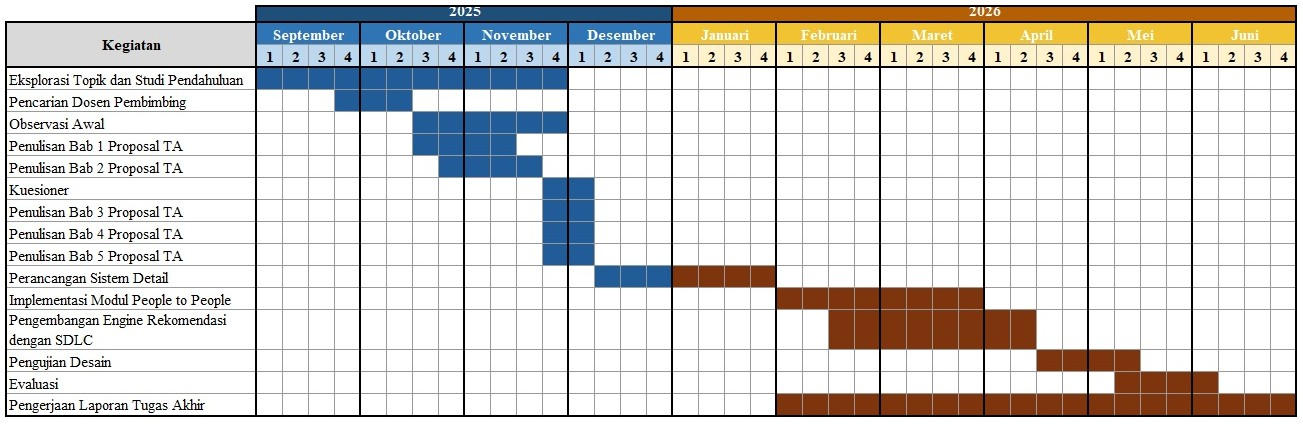
\includegraphics[width=1\textwidth]{image/51.jpg}
	\caption{Gantt Chart Rencana Pengerjaan Tugas Akhir}
	\label{gambar:51}
\end{figure}

\section{Pengujian Design}
Tahap pengujian pada Tugas Akhir ini dilakukan untuk memastikan bahwa desain sistem dan artefak yang dikembangkan telah memenuhi kebutuhan pengguna serta mampu mendukung proses pencarian rekan kolaborasi secara efektif. Pengujian dilakukan melalui dua pendekatan utama, yaitu \textit{User Acceptance Testing} (UAT) dan \textit{Usability Testing}, yang berfokus pada sisi interaksi pengguna, serta \textit{Scenario-Based Evaluation} yang digunakan untuk memvalidasi relevansi mekanisme rekomendasi berbasis \textit{Affinity-Based Matching}.

Pada tahap \textit{User Acceptance Testing} (UAT), pengujian difokuskan pada penilaian sejauh mana alur penggunaan pada modul \textit{People-to-People} telah sesuai dengan ekspektasi mahasiswa sebagai pengguna utama. Pengguna diminta menjalankan serangkaian skenario yang mencakup pembuatan dan pembaruan profil, pengaturan preferensi kolaborasi, melihat rekomendasi partner, serta melakukan interaksi dasar seperti save profile dan express interest. Melalui skenario tersebut, dievaluasi apakah fungsi-fungsi utama berjalan sebagaimana mestinya, apakah alur proses dapat dipahami dengan baik, serta apakah sistem mendukung kebutuhan mahasiswa dalam menemukan rekan kolaborasi yang relevan.

Sementara itu, \textit{Usability Testing} difokuskan pada evaluasi aspek kenyamanan dan kemudahan penggunaan antarmuka modul \textit{People-to-People}. Pada tahap ini, pengguna diminta untuk menilai kejelasan elemen antarmuka, konsistensi gaya visual, kemudahan navigasi, serta tingkat intuitivitas tampilan fitur seperti halaman rekomendasi, tampilan profil calon partner, dan komponen informasi atribut pengguna. Umpan balik yang diperoleh digunakan untuk mengidentifikasi potensi hambatan dalam penggunaan sistem dan memperbaiki desain agar lebih efisien serta lebih mudah dipahami.

Selain pengujian pada sisi interaksi, mekanisme rekomendasi berbasis \textit{Affinity-Based Matching} juga divalidasi untuk memastikan bahwa skor kecocokan yang dihasilkan bersifat relevan dan merepresentasikan kondisi nyata preferensi mahasiswa. Validasi dilakukan melalui \textit{Scenario-Based Evaluation}, yaitu pengujian yang melibatkan serangkaian skenario profil mahasiswa dan potensi rekan kolaborasi. Pengguna diminta membandingkan rekomendasi yang diberikan sistem dengan pilihan partner yang mereka anggap cocok berdasarkan intuisi atau preferensi pribadi. Hasil perbandingan ini digunakan untuk menilai apakah algoritma \textit{affinity} mampu menghasilkan rekomendasi yang sejalan dengan keputusan pengguna. Pendekatan ini membantu memastikan bahwa model kecocokan tidak hanya bekerja secara matematis, tetapi juga konsisten dengan kebutuhan dan perilaku nyata mahasiswa.

\section{Analisis Mitigasi dan Resiko}
Analisis risiko dilakukan untuk mengidentifikasi potensi hambatan yang dapat memengaruhi kelancaran proses perancangan, pengembangan, dan pengujian modul rekomendasi \textit{People-to-People} pada aplikasi kolaborasi mahasiswa. Mengingat keterbatasan waktu, sumber daya, serta ketergantungan antar tahap pengembangan, tidak semua risiko memiliki tingkat urgensi yang sama. Oleh karena itu, tugas akhir ini memfokuskan analisis pada risiko-risiko yang memiliki dampak terbesar terhadap keberhasilan sistem rekomendasi dan proses pengujian desain. Daftar risiko dan strategi mitigasi disajikan pada tabel berikut.
\begin{longtable}{@{\extracolsep{\fill}} p{1cm} p{6cm} p{8cm}}
\caption{Daftar Risiko dan Strategi Mitigasi}\label{tbl:risiko-mitigasi} \\
\toprule
\textbf{No} & \textbf{Risiko} & \textbf{Mitigasi} \\
\midrule
\endfirsthead

\caption[]{Daftar Risiko dan Strategi Mitigasi (lanjutan)} \\
\toprule
\textbf{No} & \textbf{Risiko} & \textbf{Mitigasi} \\
\midrule
\endhead

\midrule
\multicolumn{3}{r}{\textit{Bersambung ke halaman berikutnya}} \\
\bottomrule
\endfoot

\bottomrule
\endlastfoot

% ====== DATA TABEL ======
1 &
\textbf{Jadwal pengerjaan tidak sesuai rencana sehingga menghambat penyelesaian tahap desain atau implementasi modul People-to-People.} &
Menyediakan \textit{buffer time}, menetapkan prioritas pengerjaan, melakukan evaluasi progres mingguan, serta menyelesaikan komponen inti (\textit{engine} rekomendasi dan struktur data) lebih awal. \\

2 &
\textbf{User testing tidak memenuhi jumlah responden atau kualitas umpan balik rendah sehingga hasil evaluasi tidak valid.} &
Memperluas rekrutmen peserta melalui komunitas mahasiswa, menggunakan insentif ringan, serta menyediakan skenario uji yang jelas agar responden dapat memberi umpan balik yang relevan. \\

3 &
\textbf{Algoritma \textit{affinity} menghasilkan rekomendasi yang tidak akurat atau tidak konsisten.} &
Meninjau kembali bobot atribut, menguji algoritma dengan beberapa skenario realistis, melakukan \textit{parameter tuning}, serta mengadaptasi perbaikan berdasarkan \textit{feedback} pengguna pada tahap evaluasi. \\

4 &
\textbf{Integrasi \textit{engine} rekomendasi dengan modul UI People-to-People atau modul lain tidak stabil atau mengalami error.} &
Melakukan integrasi secara bertahap, menerapkan pengujian per modul, memastikan struktur data dan API konsisten, serta memperbaiki bug secepat mungkin ketika ditemukan. \\

5 &
\textbf{Desain antarmuka tidak sesuai kebutuhan pengguna sehingga mengurangi efektivitas modul rekomendasi.} &
Melakukan \textit{usability testing} pada beberapa putaran desain, memperbaiki elemen antarmuka berdasarkan umpan balik, serta tetap menerapkan prinsip UCD secara konsisten. \\

\end{longtable}

Dengan demikian, analisis risiko ini diharapkan mampu mendukung keberhasilan implementasi modul rekomendasi \textit{People-to-People} yang dikembangkan, serta meminimalkan gangguan yang dapat memengaruhi kualitas hasil tugas akhir. Upaya mitigasi yang direncanakan disusun untuk memastikan bahwa sistem rekomendasi dapat berjalan stabil, mudah digunakan, dan menghasilkan rekomendasi yang relevan bagi mahasiswa.
